
\chapter{基于深度混合强化学习的直效营销策略}

\section{研究动机}
在马尔科夫决策过程中,要求系统的状态具有马尔科夫性,即下一个时刻$S_{t+1}$仅与当前的状态$S_{t}$和当前采取行为$A_{t}$有关,与之前拥有的状态和采取的行为都无关。所以,当采用强化学习对直复营销场景进行建模时,存在的一个假设是客户的当前状态完全概括了他与营销人员在此之前的整个交互历史。也就是说客户的下一步响应情况仅与他当前的状态和营销人员采取的下一步营销行为有关,与之前的交互历史无关。但是,和很多其他现实应用所面临的问题一样,在直复营销场景中,因为客户的状态存在部分可观测性(Partial Observability)的问题,使得上述这个假设很难得到满足。

在本文的第三章中,为了更好的捕捉募捐者的状态,在进行仿真实验的时候从观测数据中提取了大量募捐者特征,而这些特征有很多是需要借助专家的领域知识或经验才能获得的。即便如此,这也只概括了客户真实状态中的部分信息。因此,在对这些场景应用强化学习之前,进行状态的推断学习是很重要的。

在像直复营销这类复杂的现实场景中,构建这种具有马尔科夫性的状态是很难的。在强化学习的研究和应用中,处理部分可观测问题最常用的方法有两种,其一是使用部分可观测的马尔科夫决策过程(Partially Observable Markov  Decision Process,POMDP)\citep{kaelbling1998planning},其二是预测状态表示法(Predictive State Representation,PSR)\citep{littman2002predictive}。POMDP虽然有着坚实的理论基础,并且已经在一些诸如机器人、人机对话等领域取得了不错的表现\citep{pineau2003point,williams2007partially},但是POMDP模型的建立需要依赖部分可观测的名义状态(Nominal State),所以系统的POMDP是很难学习的,而且需要很多专家领域的先验知识来定义隐藏状态集和观测概率集。Littman等人于2002年提出了一种新的动态系统建模方法———PSR\citep{littman2002predictive},用于处理部分可观测的问题,他的优势在于仅通过观察值序列就可以预测未来事件。尽管PSR具有很强的表示能力,并且比POMDP方法更容易从数据中学到信息,但是仍然需要大量的领域知识来设计特征和核函数。

近年来,强化学习和深度神经网络的结合取得了重大突破,并成功的应用在了游戏、围棋等领域\citep{mnih2013playing, mnih2015human},形成了一个重要的研究方向,深度强化学习。深度强化学习的成功应用除了充分发挥强化学习技术在序贯决策上的优势外,还离不开神经网络的强大作用,其作用主要包括两点。一方面利用了神经网络强大的非线性逼近能力进行值函数的逼近,更好的学习最优策略,另一方面神经网络也可以自动的进行隐状态的学习和表示,一定程度上解决状态的部分可观测问题。与上述POMDP和PSR方法不同,基于神经网络的方法可以在不依靠专家领域知识的情况下,对任何问题都可以给出隐状态的合理表示方法\citep{deng2014deep},从而解决了在实际应用中,当使用强化学习时需要人为设计隐状态的困扰

受此启发,本文针对直复营销场景中的用户状态部分可观测问题,提出使用深度强化学习方法进行解决。进一步地,从深度强化学习DQN模型出发,结合直复营销场景的时序特点,提出使用基于循环神经网络的DQN网络:DQN_RNN,另外,为了更好的学习隐藏状态的表示方法以及保证值函数逼近效果,提出了基于RNN的深度混合强化学习模型,并对网络结构进行进一步的分析和优化。

\begin{algorithm}[htbp]
 \small
 \SetAlgoLined
 \SetKwRepeat{Repeat}{repeat}{until} 
 初始化回放记忆库$D$,记忆库大小为$N$\;
 利用随机参数$\bm{\theta}$初始化Q值函数\;
 初始化Q目标值网络$\bm{\theta}^{-}$,令$\bm{\theta}^{-}=\bm{\theta}$\;
 \For((循环每个情节)){$episode=1,\cdots, M$}{
	初始化情节(episode)的第一个状态:$S_{1}$\;
	% ,通过预处理得到该状态对应的特征输入:$\phi_{1}=\phi(s_{1})$\;
	\For((初始化情节中的每一步)){$t=1,\cdots, T$}{
		以概率$\epsilon$选一个随机行为$A_{t}$\;
		如果以上小概率事件没有发生,则选择当前值函数最大的那个行为:$A_{t}=\argmax_{a}Q(S_{t},a;\bm{\theta})$\;
		在仿真器中执行行为$A_{t}$,可以得到奖赏$R_{t}$以及环境的下一步状态$S_{t+1}$\;
		% 设置$s_{t+1}=s_{t},a_{t},x_{t+1}$,预处理得到对应的特征输入:$\phi_{t+1}=\phi(s_{t+1})$\;
		将转换样本$<S_{t}, A_{t}, R_{t}, S_{t+1}>$放到回放记忆库$D$中\;
		从回放记忆库$D$中均匀随机采样一小批转换样本$<S_{j}, A_{j}, R_{j}, S_{j+1}>$\;
		判断是否是一个情节的终止状态,若是,则Q目标值为$R_{j}$,否则利用Q目标网络$\bm{\theta}^{-}$计算Q目标$R_{j}+\gamma \max_{a^{'}}Q(X_{j+1},a^{'};\bm{\theta}^{-})$\;
		使用随机梯度下降(公式$\eqref{dituxiajiangq}$)更新当前网络参数:
		更新Q值函数当前网络(MainNet)参数:$\bm{\theta}=\bm{\theta}+\triangle \bm{\theta}$\;
		每隔$C$步更新一次Q目标网络(Target)参数;即:$\bm{\theta}^{-}=\bm{\theta}$\;
	}
 }
 % 输出最终策略:$\pi(s)=\argmax_{a}Q(s,a)$\;
 \caption{DQN算法}
 \label{algo:algorithm_DQN}
 \end{algorithm}


\section{DQN_RNN模型}

\subsection{DQN模型}
 DQN算法是在Q-learning算法($\ref{algo:algorithm_2}$)的基础上改进而来,如第二章所述,主要包括以下三个方面进行改进:

 1)使用卷积神经网络进行Q值函数的逼近。2)通过经验回放(Experience Replay)机制来解决强化学习中相关性以及非静态分布的问题。3)通过独立设置目标网络(Target Net)来单独处理时间差分算法中的TD偏差,进一步降低数据之间的关联性,从而削弱收敛不稳定的问题。

\paragraph{DQN模型流程}
 从文献\citep{mnih2015human}中可以得到DQN算法的伪代码如$\ref{algo:algorithm_DQN}$所示。进一步的,可以总结出DQN算法学习过程主要包括以下几步(DQN的算法流程图如图$\ref{fig:liuchengtu_DQN}$所示):

 \begin{figure}[htbp]
\centering
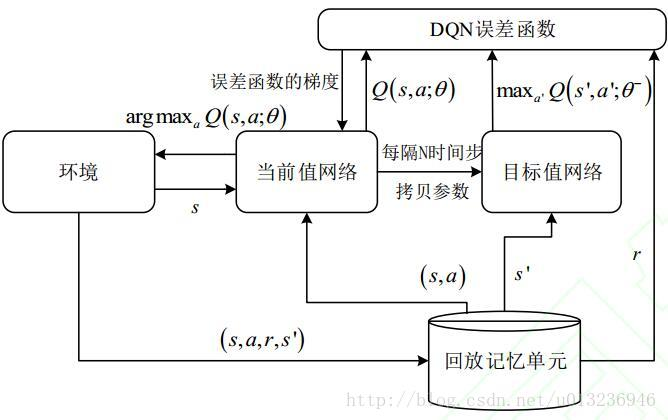
\includegraphics[width=0.9\textwidth]{liuchengtu_DQN}
\caption{DQN流程图}
\label{fig:liuchengtu_DQN}
\end{figure}
 

(1)构建回放记忆单元。在每个情节中,首先初始化第一个状态$S_{1}$,然后,在接下来的每个时间步里,按照$\epsilon-greedy$策略选择行为$A_{t}$,并在仿真器中执行$A_{t}$,即可得到对应的即时奖赏$R_{t}$和下一步的状态$S_{t+1}$,将此转换样本$<S_{t}, A_{t}, R_{t}, S_{t+1}>$放到回放记忆单元中。

(2)值函数的学习。从回放记忆单元中随机选取一小批转移样本,并分别使用当前值网络(MainNet)和目标值网络(TargetNet)计算出Q估计值 $Q(s,a;\bm{\theta})$和Q目标值$r+\gamma \max_{a^{'}}Q(s^{'},a^{'};\bm{\theta}^{-})$,然后得到损失函数$L=[r+\gamma \max_{a^{'}}Q(s^{'},a^{'};\bm{\theta}^{-})-Q(s,a;\bm{\theta})]^{2}$,并使用随机梯度下降法进行求解,以更新当前值网络MainNet的参数。
% $<S_{j}, A_{j}, R_{j}, S_{j+1}>_{j=1}^{N}$

(3)更新目标网络参数。经过若干步的训练后,将当前网络的参数拷贝给目标网络,进行目标网络的参数更新。 

(4)当DQN网络训练完毕后,将环境的当前状态$S_{t}$输入到当前值网络,便会输出DQN的动作选择策略$A_{t}=\argmax_{a}Q(S_{t},a;\bm{\theta})$。

\paragraph{DQN模型误差更新}
进一步地,DQN模型的损失函数构建过程参见图$\ref{fig:loss_DQN}$,从图中可以看出,当前值网络(MainNet)和目标值网络(TargetNet)都是关于状态$s$的网络。在进行损失函数的计算时,将状态$S_{t}$输入当前值网络,并根据行为$A_{t}$从当前值网络找到当前的Q估计值,然后将状态$S_{t+1}$带入目标值网络,得出Q目标值,Q目标值和Q估计值的均方误差即为当前的损失。

% 在DQN中增强学习Q-Learning算法和深度学习的SGD训练是同步进行的
\begin{figure}[htbp]
\centering
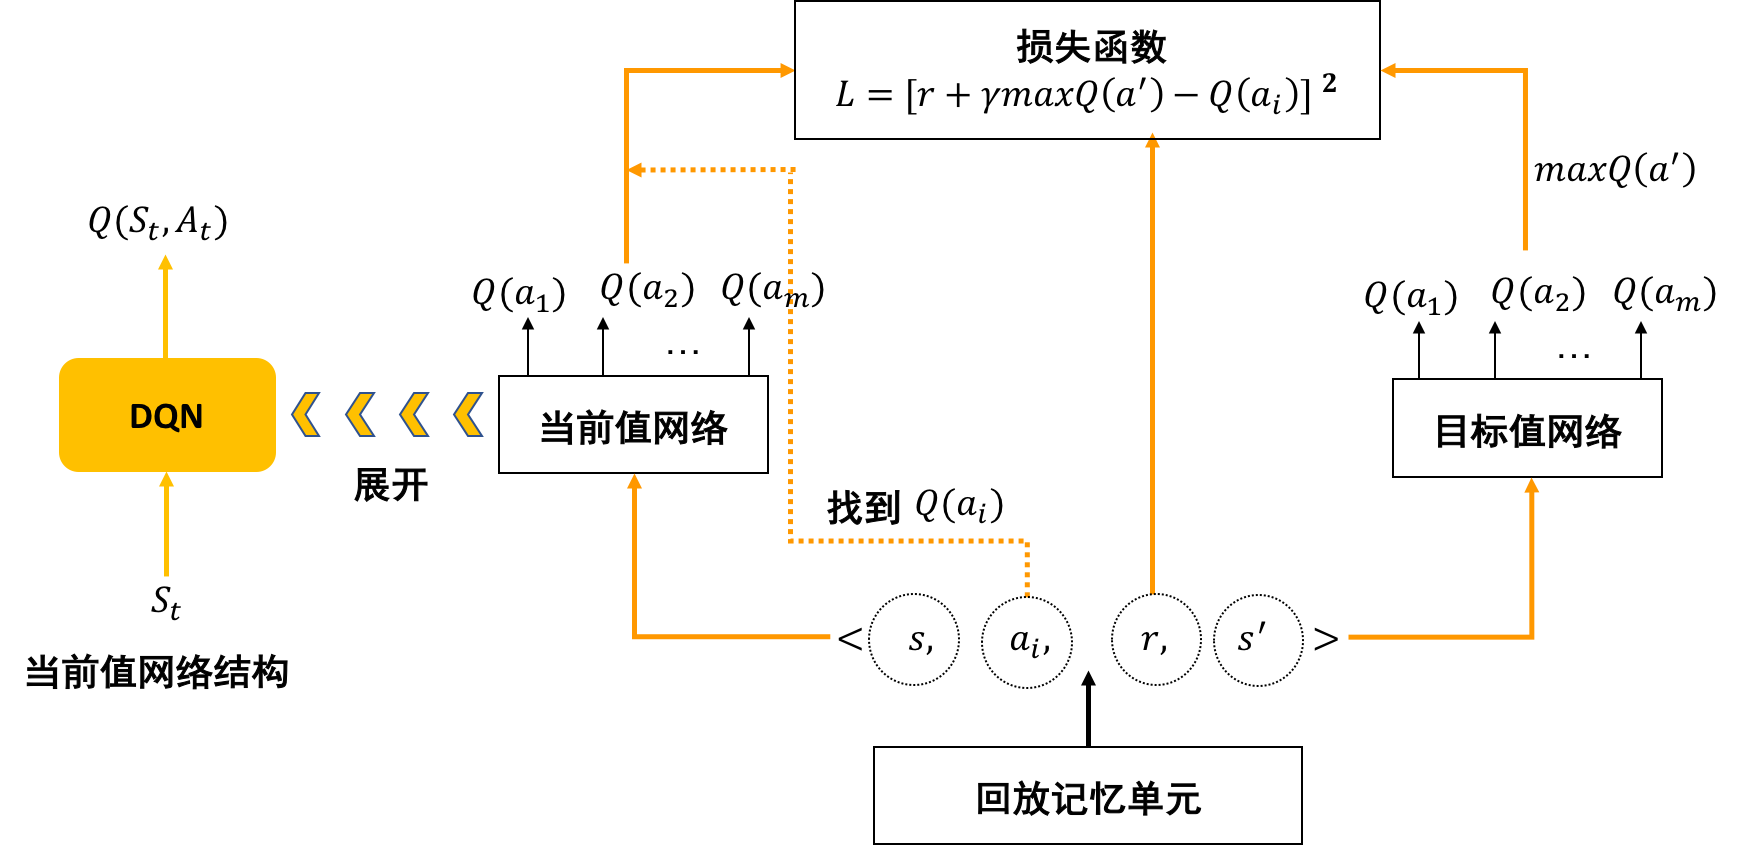
\includegraphics[width=0.6\textwidth]{loss_DQN}
\caption{DQN损失函数构造}
\label{fig:loss_DQN}
\end{figure}

\paragraph{DQN基准模型}
可以直接将DQN模型用于直效营销的场景的建模中。具体做法就是将客户的观测值$O_{t}$当作状态$S_{t}$,客户产生的利润当作即时奖赏$R_{t}$,营销人员采取不同类型营销方式作为行为$A_{t}$。在客户和营销人员的不断交互中形成转移样本$\{<O_{t}, A_{t}, R_{t}, O_{t+1}>\}_{t=1,2,\cdots}$,再按照上述DQN算法$\ref{algo:algorithm_DQN}$去训练网络的参数。经过若干次的训练后,当得到一个近似最优的Q值函数时,带入客户的状态,就可以按照贪婪的方式从值函数中选择最佳的营销行为$\argmax_{a}Q(s,a)$。

图$\ref{fig:dqn_crm}$为DQN当前值网络简化的网络示意图。其中,$O_{t}$为用户的观测值,$Q(S_{t},A_{t})$为在$t$时刻时,执行行为$A_{t}$所的到的Q估计值。需要注意的是,在使用DQN模型进行训练时,前一个输入和后一个输入之间是没有关系的。
\begin{figure}[htbp]
\centering
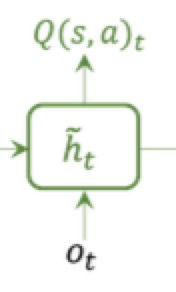
\includegraphics[width=0.2\textwidth]{dqn_crm}
\caption{DQN当前值网络结构}
\label{fig:dqn_crm}
\end{figure}

\subsection{基于RNN的DQN模型}
在将DQN模型应用到Atari游戏中时\citep{mnih2013playing},DeepMind团队之所以会选择卷积神经网络CNN作为Q函数逼近器,是因为在CNN结构中,通过卷积操作和池化操作可以大幅度降低网络参数,从而加快网络的训练。此外,CNN网络还非常善于抽取位置不变的特征,特别适合图像这类网格型结构的数据,因此广泛应用在图像识别领域。在视频游戏中,由于输入是图像,所以使用CNN结构的神经网络逼近值函数的效果就会很好。

但是,在CNN网络中假设输入是一个独立的没有上下文联系的单位,即前一个输入和后一个输入是没有关系的,所以CNN无法对时间序列上的变化进行建模。而样本出现的时间顺序对于自然语言处理、语音识别、手写体识别等应用非常重要。为了适应这种需求,就出现了另一种神经网络结构——循环神经网络(Recuurent Neural Network, RNN)

 \paragraph{RNN网络}
RNN是一种对序列数据建模的神经网络,可以连接先前的信息到当前的任务上来。具体的做法是:网络会对前面的信息进行记忆存储并应用于当前输出的计算中,即隐藏层之间的节点不再无连接而是有连接的,并且隐藏层的输入不仅包括输入层的输出还包括上一时刻隐藏层的输出。图$\ref{fig:rnn}$是一个RNN模型的简化结构展开图。
\begin{figure}[htbp]
\centering
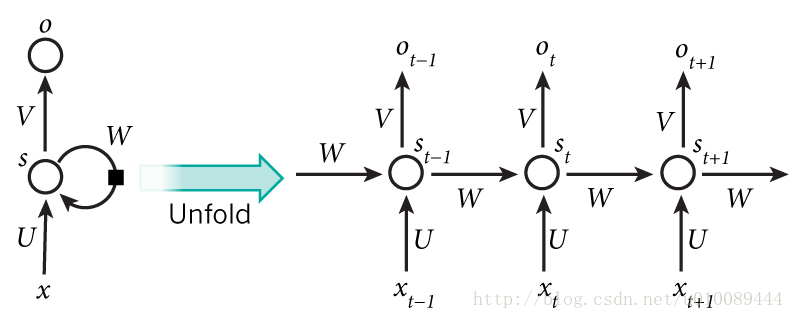
\includegraphics[width=0.8\textwidth]{rnn}
\caption{RNN模型的简化结构展开图}
\label{fig:rnn}
\end{figure}

在图$\ref{fig:rnn}$中,$x_{t}$表示$t$时刻的输入;$s_{t}$表示$t$时刻的隐藏层的记忆值(Memory),它基于上一时刻的隐状态和当前输入得到;
% \begin{equation}
% \begin{aligned}
% s_t=f(U x_{t}+W s_{t-1})
% \end{aligned}
% \end{equation}
% 其中,$f(\cdot)$一般是非线性的激活函数;
% 在计算$s_{0}$时,即第一个单词的隐藏层状态,需要用到$s_{−1}$,但是其并不存在,在实现中一般置为0。
$o_{t}$表示$t$时刻的输出。$U$是输入层到隐藏层的权重矩阵,$V$是隐藏层到输出层的权重矩阵,权重矩阵$W$就是隐藏层上一次的值作为这一次的输入的权重。需要注意的是:在传统神经网络中,每一个网络层的参数是不共享的,而在RNN中,所有层次均共享同样的参数,
% 其反应出RNN中的每一步都在做相同的事,只是输入不同,
因此大大地降低了网络中需要学习的参数。网络在$t$时刻接收到输入$x_{t}$之后,隐藏层的值是$s_{t}$,输出的值是$o_{t}$。
% 特别的,$o_{t}$的值不仅仅取决于$x_{t}$,还取决于$o_{t-1}$。
我们可以用下面的公式来表示循环神经网络的计算方法:
\begin{equation}
\label{rnn_1}
\begin{aligned}
o_{t}=g(V s_{t})
\end{aligned}
\end{equation}
\begin{equation}
\label{rnn_2}
\begin{aligned}
s_{t}=f(U x_{t}+W s_{t-1})
\end{aligned}
\end{equation}

式\eqref{rnn_1}是输出层的计算公式,输出层是一个全连接层,也就是它的每个节点都和隐藏层的每个节点相连。$V$是输出层的权重矩阵,$g$是激活函数。式\eqref{rnn_2}是隐藏层的计算公式,它是循环层。$U$是输入$x$的权重矩阵,$W$是上一次的值作为这一次的输入的权重矩阵,$f$是激活函数。从上面的公式我们可以看出,循环层和全连接层的区别就是循环层多了一个权重矩阵$W$。如果反复把式$\eqref{rnn_2}$带入到式$\eqref{rnn_1}$,我们将得到:
\begin{equation}
\label{rnn_3}
\begin{aligned}
o_{t}&=g(V s_{t})\\
&=V f(U x_{t}+W s_{t-1})\\
&=V f(U x_{t}+W f(U x_{t-1}+W s_{t-2}))\\
&=V f(U x_{t}+W f(U x_{t-1}+W f(U x_{t-2}+W f(U x_{t-3}+\cdots)))\\
\end{aligned}
\end{equation}

从式\eqref{rnn_3}可以看出,循环神经网络的输出值$o_{t}$,是受前面历次输入值$x_{t}$、$x_{t-1}$、$x_{t-2}$、$x_{t-3}$、$\cdots$影响的,这就是为什么循环神经网络可以往前看任意多个输入值的原因,也是它为什么善于按序列对单元进行建模的原因。

RNN的训练方法是采用基于时间的反向传播算法(BackPropagation Through Time, BPTT),具体的更新方法和BP更新方法相同。
% 但是,在处理较长序列的时候, RNN不能得到较好的性能。一个主要原因是,RNN在训练中如果向前考虑的很远的时候,会导致对应的误差项的值增长或者缩小的非常快,就会很容易发生梯度爆照或者梯度消失的现象,这导致训练时梯度不能在较长序列中一直传递下去,从而使RNN无法捕捉到长时间距离的信息。由此,提出了长短时记忆网络(Long  Short-Term Memory,LSTM)。

% 因为原始RNN的隐藏层只有一个状态,它对于短期的输入非常敏感,LSTM在此基础上增加了一个状态,让它保存长期的状态,从而解决了传统RNN无法处理长距离依赖的问题。新增加的状态称为单元状态(Cell State)。因为篇幅的限制,关于LSTM的原理在此不表,详见文献\citep{hochreiter1997long}。
 \paragraph{DQN_RNN}
 因为RNN网络在时序变化问题中的强大建模能力,为了更好的将强化学习应用在序列相关问题中,所以,出现了很多对基于RNN网络的DQN模型的研究\citep{hausknecht2015deep,narasimhan2015language}。在这些研究中,作者普遍采用的做法是,将DQN模型中的CNN网络替换成了RNN网络,希望通过对数据序列中存在长时依赖性的奖赏信息进行建模,来更好的处理状态部分可观测的问题\citep{bakker2002reinforcement,hausknecht2015deep,lin1993reinforcement,narasimhan2015language},以达到更好的函数逼近效果。经过实验发现,在文本、语音等序列相关问题上确实取得了比传统基于CNN网络的DQN模型更好的表现。

 同样地,在直复营销场景中,客户和营销人员的交互也是一个随时间而不断发生变化的过程。因此,如果使用基于RNN的DQN模型(记作DQN_RNN)对直复营销场景进行建模,可以充分利用RNN的长时依赖性更好的学习客户的状态表示方法,进而达到更好的策略学习的目的。

 结合文献\citep{hausknecht2015deep,narasimhan2015language}所设计的模型,可以得到DQN_RNN当前值网络的简化结构示意图$\ref{fig:rl_rnn}$。对应到直复营销场景中,$O_{t}$表示$t$时刻客户的观测信息,$\tilde{h}_{t}$为$t$时刻客户的隐状态信息,$Q(S_{t}, A_{t})$表示在$t$时刻,当状态$S_{t}$等于$\tilde{h}_{t}$且采取行为$A_{t}$时的Q估计值。因为隐状态$\tilde{h}_{t}$是关于上一时刻隐状态$\tilde{h}_{t-1}$和当前观测$O_{t}$的函数,所以,Q网络也是关于当前观测$O_{t}$和上一时刻隐状态表示方法$\tilde{h}_{t-1}$的函数。当Q值网络训练完毕后,以贪婪的方式选择最优的行为。

 \begin{figure}[htbp]
 \centering
 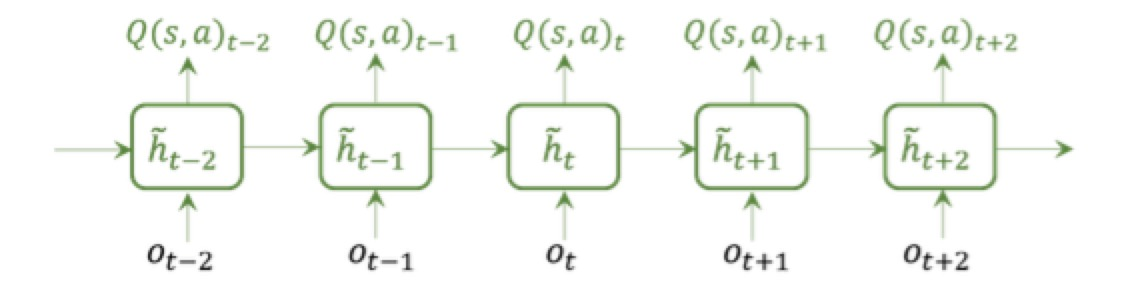
\includegraphics[width=1.0\textwidth]{rl_rnn}
 \caption{DQN_RNN当前值网络结构}
 \label{fig:rl_rnn}
 \end{figure}

 另外,与DQN模型的流程图$\ref{fig:liuchengtu_DQN}$相比,DQN\_RNN模型的流程图的当前值网络和目标值网络变成了RNN网络,并且回放记忆单元中存储的是有固定步长的序列,而不是独立的状态转移样本。在构建回放记忆单元时,需要模型和环境持续的进行固定步长的交互来形成一个序列样本。同样,从回放记忆单元中抽取批样本时,也是以序列样本的形式抽取,其他部分和图$\ref{fig:liuchengtu_DQN}$相同。损失函数的构造和DQN模型的损失函数构造方式($\ref{fig:loss_DQN}$)相同。

\section{基于RNN的深度强化学习混合模型}
在上述DQN\_RNN的模型中,利用RNN网络的长时依赖性,希望可以在时间变化的序列问题上更好的捕捉到状态的隐藏信息,进而在学习的过程更好的逼近Q值函数。所以,在RNN网络的优化过程中同时肩负着两个任务:

(1)Q值函数的逼近(策略学习)

(2)序列的长时依赖性学习(隐状态表示方法的学习)。

而对于只有一个RNN网络的DQN模型来说,同时进行这两个任务,往往会在实际的应用中导致学习效果不佳。在本节中,针对以上问题,提出了基于两个神经网络的混合强化学习模型。另外,根据训练方式的不同,又分为RNN+DQN$^{*}$两网络独立模型、1-RNN+DQN一步混合模型和2-RNN+DQN两步混合模型。

\subsection{两网络独立模型}
如上文所述,对于只有一个RNN循环神经网络的DQN\_RNN模型来说,在网络优化的过程中,同时兼具序列的长时依赖性学习和长期最大化策略的学习是比较困难的。那么,一个很自然的想法是,使用两个网络对以上两个任务分别进行学习,由此得到两网络独立模型。

本文的想法是:使用RNN和DQN两个网络进行训练。具体地,首先,进行RNN网络的训练:利用在交互过程中产生的监督数据,比如即刻奖赏、观测值等信息,通过RNN网络来对序列的长期依赖性进行建模,以单独的学习隐藏状态的表示方法。待RNN网络学习完毕后,进入DQN网络的训练:将观测值输入到学好的RNN网络,再将RNN网络学习到了隐状态信息作为DQN网络的输入状态,然后依靠DQN网络强大的非线性表达能力逼近Q值函数,以进行更充分的策略学习,达到最大化累积奖赏的目的。

其中,第一个部分属于监督学习过程,可以充分发挥RNN网络对时间序列建模的优势,第二个部分属于强化学习过程,可以充分发挥DQN网络对值函数学习的优势,通过这两个网络的优势互补,可以进行更有效的强化学习。将此模型记作:RNN+DQN$^{*}$

两网络独立模型的结构图如图$\ref{fig:rnn+dqn}$所示。左边部分为RNN网络的监督学习过程,其中,$O_{t}$是观测值,$h_{t}$是藏状态信息,$O_{t+1}^{'}$是$t+1$ 时刻的预测的观测值,$R_{t}$。右边为DQN网络的强化学习过程,其中,$O_{t}$是观测值,$h_{t}$是藏状态信息,$Q(S_{t},A_{t})$是$t$时刻Q的估计值,它是一个关于隐状态$h_{t}$的函数。

在测试阶段,将上一时刻的隐状态信息和这一时刻的观测值作为RNN的输入,然后再将产生的隐状态信息输入到已经学习好的Q值网络中,以贪婪的方式选择最优的行为。

同样,RNN+DQN$^{*}$的误差构造也分为两个部分,如图$\ref{fig:rnn+dqn}$所示。左边为RNN监督学习的误差构造过程,主要是利用预测的下一步观测值和预测的奖赏值与真实的下一步观测值和奖赏值来构造损失函数训练RNN网络。右边为DQN网络的误差构造过程,虽然都是和之前DQN网络的误差构造方法相同,都是利用Q目标值和Q估计值的均方误差作为损失函数,但是两个网络的输入从观测值变成了RNN的隐状态值。

\begin{figure}[htbp]
\centering
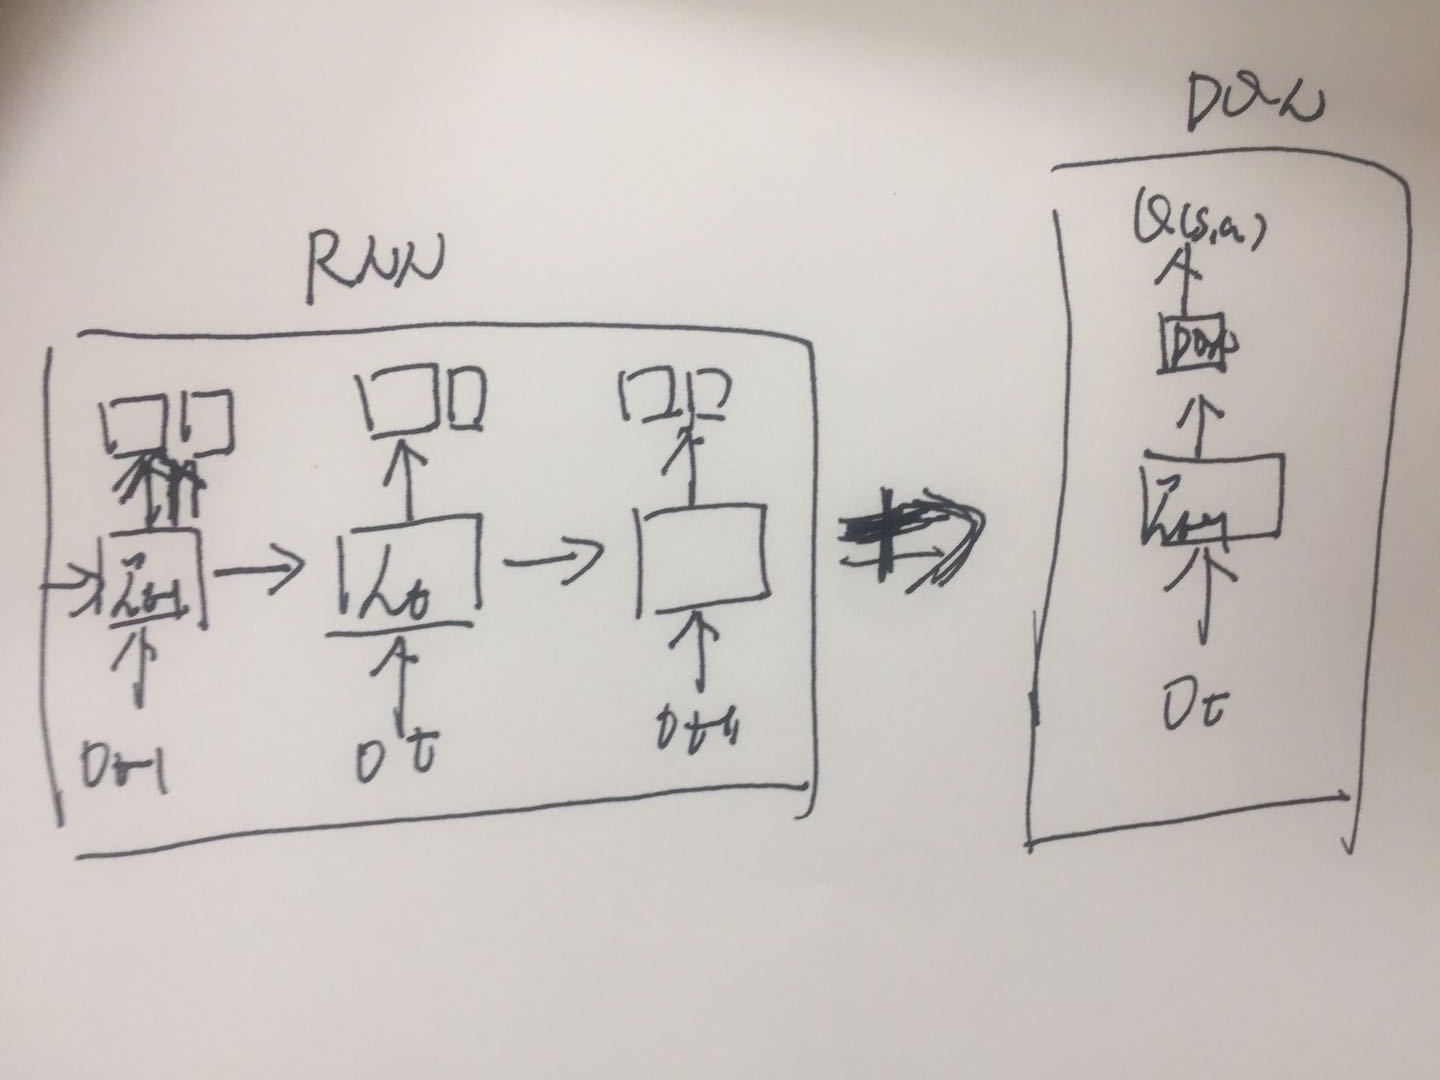
\includegraphics[width=0.8\textwidth]{rnn+dqn}
\caption{RNN+DQN$^{*}$网络结构图}
\label{fig:rnn+dqn}
\end{figure}

\subsection{一步混合模型}
在RNN+DQN$^{*}$模型中,虽然充分利用了RNN网络和DQN网络各自的优点,但是仍然存在一个问题:两个网络的优化过程被完全割裂开来,这样造成的一个后果就是我们很难知道已经训练好的RNN网络是否可以让DQN网络学到好的Q值函数,或者说很难知道RNN网络训练到什么程度才可以让DQN更好的产生一个Q值函数。

基于这个想法,本节提出一种联合训练的方法。让RNN网络在每学到一个隐状态表示方法后,就立刻让DQN网络以此隐状态表示方法产生的输出作为状态输入进行学习,两个网络交替进行更新,直到DQN网络学到一个好的Q函数,就停止学习。将这种模型称为一步混合模型1-RNN+DQN。

1-RNN+DQN的网络结构如图$\ref{fig:rnn_dqn}$所示,其中,$O_{t}$是观测值,$h_{t}$是隐藏状态,$O_{t+1}^{'}$是预测的$t+1$时刻的观测值,$R_{t}$是预测的$t$时刻即时奖赏值,$Q(S_{t},A_{t})$是$t$时刻预测的Q值。蓝色部分对应着RNN网络的监督学习部分,红色部分对应着DQN的强化学习部分。同样地,DQN的输入是RNN模型的隐状态。只不过在参数优化的过程中,两个网络依次交替进行。

具体来说,在训练阶段,使用联合训练的方法。首先,在每一个时刻,通过预测下一步的观测值和即时奖赏值来训练RNN网络,然后将此时训练过程中产生的隐状态作为DQN网络的输入,再通过DQN网络来逼近学习Q值函数。以上这两个步骤在随机梯度的迭代过程中依此交替的进行。在测试阶段,与DQN\_RNN模型类似,将环境观测信息输入RNN网络,然后将RNN网络产生的隐藏信息作为输入状态导入到训练好的Q值网络中,以贪恋的方式选择最优行为。

特别需要强调的是,与文献\citep{hausknecht2015deep,narasimhan2015language}中所提出的模型不同的是,在训练的过程中,
使用监督信号来学习隐状态的信息,并且将监督学习的误差反向传播到RNN网络的头部,但是,强化学习的误差信号只反向传播到RNN网络的隐藏层,并不参加RNN的训练。如图$\ref{fig:rnn_dqn}$所示,1-RNN+DQN模型的误差构造过程和RNN+DQN$^{*}$的误差构造过程类似,只是没有没有分开进行,而是依次交替进行。

因为在1-RNN+DQN模型的学习过程中,RNN网络和DQN网络按照上述训练方法依次进行,期间没有发生网络结构的变化,因此我们称之为一步混合模型。
\begin{figure}[htbp]
\centering
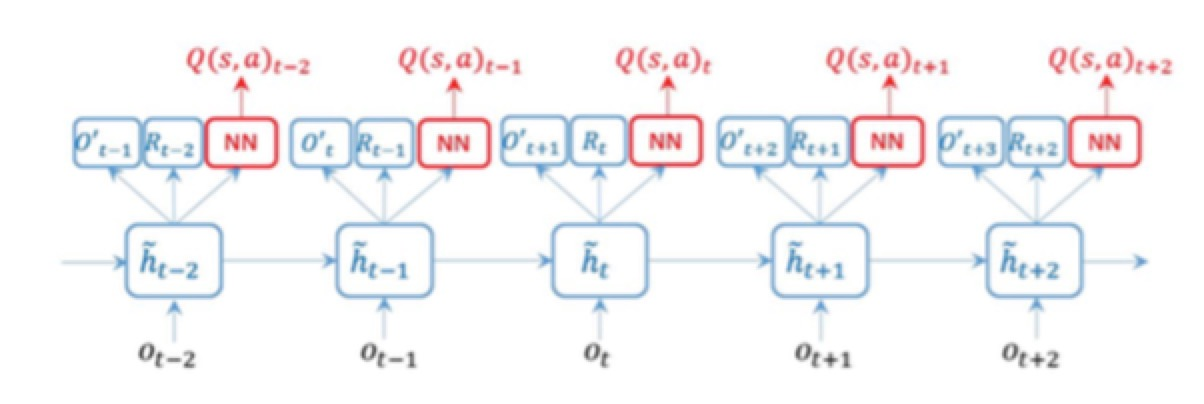
\includegraphics[width=1.0\textwidth]{rnn_dqn}
\caption{1-RNN+DQN模型结构图}
\label{fig:rnn_dqn}
\end{figure}

\subsection{两步混合模型}
在1-RNN+DQN模型中,通过使用联合训练的方法,我们可以更容易的为DQN网络的训练找到合适的RNN网络模型,以使得更好的逼近Q值函数。但是,从[图]中可以清晰的看出:在RNN网络训练的过程中,监督信号的误差传递到了RNN的头部,而在DQN网络的训练过程中,误差信号只传递到RNN的隐藏层。也就是说两个网络之间并没有进行误差的传递。这样会引起一个问题:

最初的目标是希望利用模型来学习关于观测值$o_{t}$的Q值函数,但是这种网络结构割裂了Q值函数和观测值之间的关系,导致我们在训练DQN网络的时候必须完全信任RNN网络关于隐状态的表达能力的,而无法直接接触到观测值。又因为针对RNN网络
% 的隐状态表达能力
的学习只用到了观测值和奖赏信息,并没有利用Q值信息。所以,在1-RNN+DQN模型训练的最后几个循环中,如果抛弃监督学习的过程,而将Q值的误差信息反向传播到RNN网络的头部,来同时更新RNN网络和DQN网络,进行参数的整体微调,就可以将观测值和Q值函数联系了到一起,期望会在一定程度上提升模型的效果。

所以,基于以上的想法,本节提出了两步混合模型,记为2-RNN+DQN。如图$\ref{fig:2-rnn-dqn}$所示,2-RNN+DQN模型在训练时共分为两个阶段,第一阶段,按照1-RNN+DQN的方法进行训练,学习到两个网络的参数向量$\bm{\theta}^{'}$和$\bm{\theta}^{''}$;第二阶段,将RNN网络的隐藏层和DQN网络的输入层连接起来,组成一个新的网络结构$[\bm{\theta}^{'},\bm{\theta}^{''}]$,新的网络的输入是观测值,输出是Q函数。通过这种方式,便可以在第二阶段将Q值函数的误差反向传播到RNN头部,来进行整体参数的微调。在测试阶段,将观测值输入到第二阶段新的网络结构中,通过贪婪的方式从Q值函数中选择最佳的行为。

% 训练时两个阶段训练时间应该如何把握。本实验采用的方法是将训练数据集按照8:2的比例分成两份,第一份用于第一阶段的训练,第二份用于第二阶段的训练。

\begin{figure}[htbp]
\centering
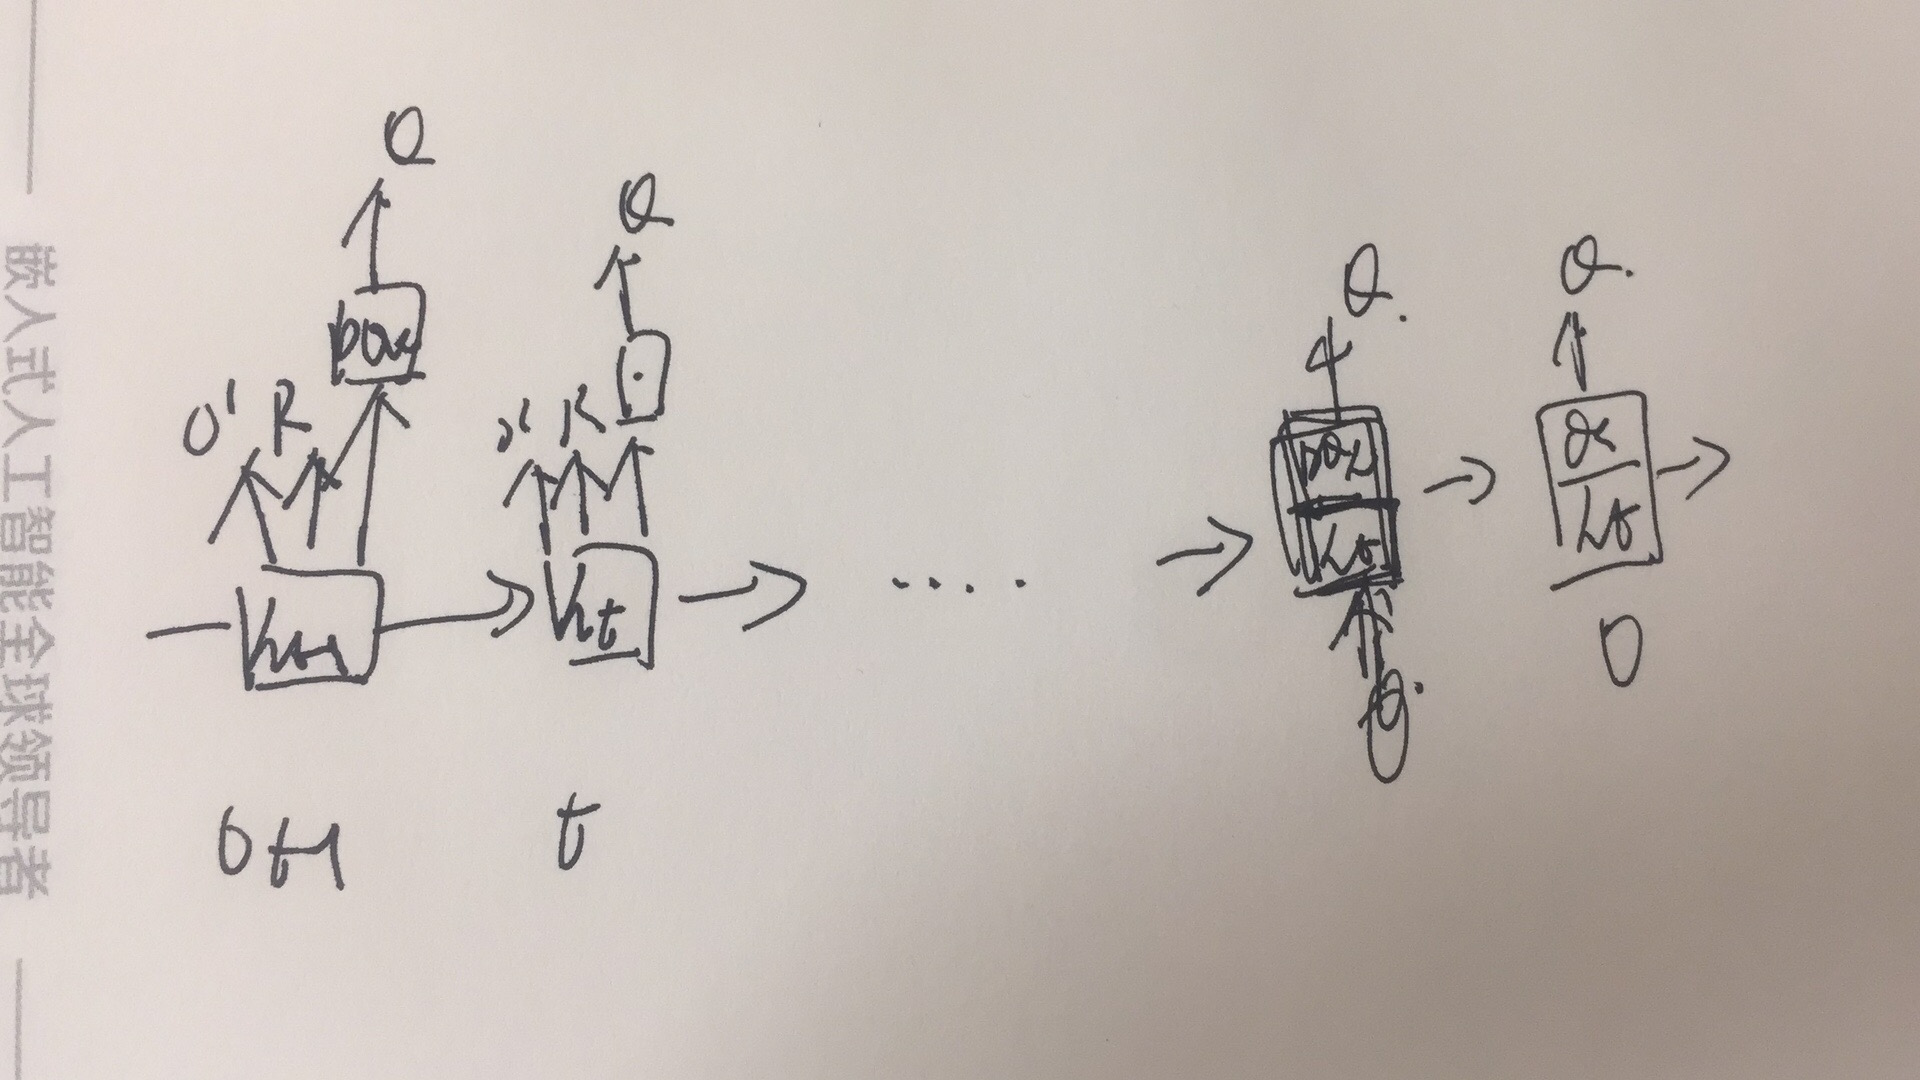
\includegraphics[width=1.0\textwidth]{2-rnn-dqn}
\caption{rnn-dqn框架}
\label{fig:2-rnn-dqn}
\end{figure}

\section{实验仿真}


\subsection{数据集}
本节,仍然选择使用UCI数据库中关于直邮营销著名的公开数据集KDD-CUP 1998\footnote{https://kdd.ics.uci.edu/databases/kddcup98/kddcup98.html}。但是,在数据特征的选择上,和第三章不同。

将原始数据集中每个募捐者的交互序列看成一个含有23步的时间序列,可表达为:$<O_{1},A_{1},R_{1},\cdots,O_{22},A_{22},R_{22},O_{23}>$,当使用CNN网络和DQN网络进行训练时,其输入为当前的观测值$O_{t}$,当涉及RNN网络的训练时,其输入为一个观测序列$<O_{1},O_{2},\cdots,O_{22},O_{23}>$
其中:

(1)$O_{t}$:表示每个募捐者的当前观测特征值。是从第三章的用户特征里取五维所组成的向量,如表~\ref{tab:obser_donors4}所示:
\begin{table}[htbp]
  \centering
  \caption{捐助者特征的选取}
  \label{tab:obser_donors4}
  \begin{tabular}{cl}
    \toprule
      特征 & 描述 \\
    \midrule
      age & 捐助者的年龄 \\
      income & 捐助者的收入 \\
      frequency & 该捐助者捐助的频率\\
      ramntall & 捐助的总金额 \\
      recency & 距离上次捐助的时间 \\
      % nrecproms & 之前六个月里,给该捐者者发送直邮营销的次数\\
      % nrecgifts & 之前六个月里,捐助者捐助的次数\\          	  
    \bottomrule
  \end{tabular}
\end{table}

(2)$A_{t}$:需要特别注意的是,本节的行为选取和第三章不同,因为在KDD-CUP 1998的数据库中,包含11种不同的邮件类型,所以可以当作11个不同的行为,加上一个不进行直邮营销这一行为,所以本章可选择的行为集合中一共有12个行为。所以,本章试验的目的就变成了,PVA采取什么样类型的邮寄行为,可以使的所获得的长期收益最大化。

(3)$R_{t}$:$R_{t}$表示执行行为$A_{t}$带来的奖赏,和第三章一样,使用PVA从捐助者获得的利润作为对应的奖赏信息。

\subsection{仿真环境}
\paragraph{仿真环境构造}
本章所构造的仿真环境和第三章仿真环境的构造原理大致相同。不同的是,预测每个捐助者响应概率的模型$P(s,a)$和产生奖赏信息的模型$A(s,a)$均使用的RNN网络来进行预测,期望通过RNN网络的长时依赖性来获得更准确的响应模型和获得的奖赏。

当有了模型$P(s,a)$和$A(s,a)$,我们可以使用如下过程来构建马尔科夫决策过程。

(1)给定状态$s$和行为$a$下的即时奖赏$R(s,a)$可以通过这两个模型得到:以$P(s,a)$的概率来掷一枚硬币,并以此来判断捐助者是否会产生反馈。即:出现正面的概率为$P(s,a)$表示捐助者会产生反馈,出现反面的概率为$1-P(s,a)$表示捐助者忽略掉了本次募捐邮件,不会产生任何反馈信息。如果没有出现反馈,那么捐助额为$0$,如果产生了反馈,那么用户的捐助金额为$A(s,a)$。即时奖赏$R(s,a)$等于捐助额减去邮寄的成本。

(2)状态转移方程也可以通过使用这两个模型计算每一个状态特征的变化情况而得到。比如:如果PVA采取的行动为1,numprom的值就会加1,否则保持不变;同样的,如果上述掷硬币的方式出现正面朝上,那么ngiftall的值就会加1,否则保持不变;有了这两个值(numprom,ngiftall),那么frequency的值也就可以计算出来了。类似的,其他状态特征也是通过这种方法计算的到的。

\paragraph{仿真评估方法}
有了上述马尔科夫决策过程的模型和状态转移方程,就可以使用如下的方式来构建我们的评估实验。

(1)首先,随机选择一定数量规模(5000)的捐助者,并设置他们的初始状态。本实验中将所选择的捐助者的初始状态设置为第7个营销活动时的状态。

(2)然后,使用学习好的强化学习模型输出策略:对每个捐助者是否应该采取营销行为。

(3)最后,使用模型$P(s,a)$和$A(s,a)$,可以得到预估的即时奖赏以及下一时刻的状态。记录这些得到信息,然后进入下一次的邮寄决策中。

就这样,按照上述的三个步骤,每循环一次就会模拟一次虚拟的直邮营销的过程。本节实验中,重复循环20次,就得到了20次的模拟直邮效果。

\subsection{仿真结果}

(1)长期收益

 首先比较以上六个模型在20次模拟直邮中的长期总收益,以下为六个模型的网络结构以及参数。
 
 \begin{table}[htbp]
  \centering
  \caption{网络结构参数}
  \label{tab:wangluojigoucanshu}
	% \begin{tabular}{p{0.9\columnwidth}} 
  \begin{tabular}{llp{10cm}}  
    \toprule
      序号 &模型 & 结构及参数描述 \\
    \midrule
      1 &RNN &一个输入层,一个隐藏层,一个输出层。其中:batch大小:512,隐藏层神经元个数:128 ,学习率:0.001\\
      2 &DQN & 两个卷积层,第一个卷积层(strides=1, patch = 2, padding='SAME', 卷积核:32)第二个卷积层(strides=2, patch = 2, padding='SAME', 卷积核:64),两个全联接层,激活函数:relu,学习率:0.001,batch大小:512\\
      3 &DQN_RNN &一个RNN网络,参数同1 \\
      4 &RNN+DQN$^{*}$ & 一个RNN网络,一个DQN网络,参数同上1,2\\
      5 &1-RNN+DQN & 一个RNN网络,一个DQN网络,参数同1,2\\
      6 &2-RNN+DQN & 一个RNN网络,一个DQN网络,参数同1,2 \\
      % nrecproms & 之前六个月里,给该捐者者发送直邮营销的次数\\
      % nrecgifts & 之前六个月里,捐助者捐助的次数\\          	  
    \bottomrule
  \end{tabular}
\end{table}

 从原始数据集中抽取10000个捐助者序列分别进行以上模型的训练,然后将抽取的样本按照1:4的比例分割成训练集和测试集。进行20波(epoch)的训练,并在每波训练完毕后,按照上述方法进行仿真试验,评估模型的质量,并记录每波模型输出策略的利润值。每组试验运行5次,并取这5次试验在每波中的平均值作为最终的结果。表[]展示上述六个模型在第20波输出策略的总收益。图[]展示了20波训练过程的模型训练情况,其中在2-RNN+DQN模型中,在最后五波中的后10个batch进行两步训练。

(2)不同数据的收据搜集方式

 为了考察不同数据搜集方式对模型试验结果的营销,本部分考虑利用仿真环境重新构建数据集。

 具体地,随机抽取10000个捐助者的序列数据,然后按照1:4的比例分割成训练集和测试集。取训练集中的捐助者的初始状态,然后从行为集合中随机的选取行为,并在仿真环境中执行,得到捐助者的下一状态和此时的奖赏信息。将次作为捐助者的第一时刻的交互数据,按照这种方式,重复进行23次,同样得到了8000个捐助者含有23个时间步的交互序列。

 然后按照上述的试验方法进行试验,同样5次的试验,每次试验20波,然后去最后一次试验最后一波策略的平均值作为最终各模型在次数据集下的策略结果。

 正确的探索对于学习良好的政策是必要的,从图[]中可以清楚的看到,采用随机选取策略的方式得到的收益明显大于按照pva给定的数据集训练所得的结果。这在一定程度上说明了,PVA的实际数据收集政策似乎是确定性的,同一步骤对所有捐助者采取同样的行动。因此,这个数据集很少或根本没有探索。 

 另外,从RNN和CNN网络输出的结果来看,因此强化学习算法比缺乏监督学习算法更容易受到缺乏探索的影响,因为强化学习在学习的过程中试图去预测将来会发生什么,探索的越少,对强化学习来说就会引入更多的误差,这与图[]所示的结果一致。

(3)不同训练规模

在最后一组实验中,通过改变了数据大小,看它是如何影响每个模型的性能的。从原始数据中随机的选取5000,10000,20000和50000个捐助者的信息分别进行试验。同样按照上述所示的方法进行训练,从表中可以清晰的看到随着数据量的提升,其结果并没有很大的变化,这说明了小数据集(5000条样本序列)同样足以产生高效的营销策略。


\section{本章小结}
本章为了解决直效营销的场景的客户生命周期最大化和状态部分可观测的问题,研究了基于RNN的深度强化学习混合模型。首先介绍场景特点,阐明本章采用基于RNN的深度强化学习的出发点,然后介绍通过介绍先有的DQN网络和DQN\_RNN网络,并分析其在解决此类问题中存在的学习能力不足的问题,提出了基于RNN的深度强化学习混合模型,并在此基础上根据网络结构的不同,提出了R两网络独立模型NN+DQN_RNN$^{*}$、一步混合模型1-RNN+DQN\_RNN和两步混合模型2-RNN+DQN\_RNN,加之之前介绍的三个基准模型DQN、RNN以及DQN_RNN,一共提到了针对直效营销场景的六种模型,第五章会对他们依次进行试验分析。